\subsection{UC5 - Scelta della \glo{visualizzazione}}
\textbf{IMMAGINE DA SISTEMARE}
\begin{figure}[h]
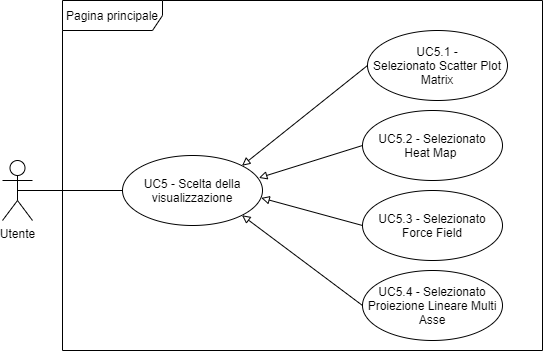
\includegraphics[width=\linewidth]{Section/Images/UC5.png}
\centering
\caption{UC5 - Scelta della visualizzazione}
\end{figure}
\begin{itemize}
	\item \textbf{Attore primario}: Utente;
	\item \textbf{Precondizioni}: L'utente ha caricato dei dati nel sistema e ha selezionato le dimensioni da utilizzare [UC2].
	\item \textbf{Postcondizioni}: Viene mostrata la visualizzazione scelta, con possibilità di personalizzazione [UC6]. La scelta viene salvata nel sistema.
	\item \textbf{Scenario principale}: L'utente seleziona la visualizzazione che vuole utilizzare tra quelle disponibili.
	%\item \textbf{Generalizzazioni}: L'utente seleziona una delle seguenti opzioni:
	%	\begin{enumerate}
	%		\item \glo{\textit{Scatter Plot Matrix}} [UC5.1];
	%		\item \glo{\textit{Heat Map}} [UC5.2];
	%		\item \glo{\textit{Force Field}} [UC5.3];
	%		\item \glo{\textit{Proiezione Lineare Multi Asse}} [UC5.4].
	%	\end{enumerate}

\end{itemize}